\documentclass[10pt,a4paper]{article}

\usepackage[a4paper,margin=1cm, bottom=1cm]{geometry}
\usepackage{tikz}
\usepackage{xcolor}
\usepackage{graphicx}
\usepackage{fontspec}
\usepackage{enumitem}
\usepackage{fontawesome5}
\usepackage[none]{hyphenat}
\usepackage{titlesec}

\setmainfont{Arial} % You might need to change this depending on your OS fonts, like Arial or TeX Gyre Heros

\pagestyle{empty}

% Colors
\definecolor{mainblue}{HTML}{6389BA}
\definecolor{textgray}{HTML}{7A7A7A}
\definecolor{darkgray}{HTML}{404040}
\definecolor{lightgray}{HTML}{E0E0E0}

% Section formatting to restore the "File Outline" panel in Overleaf cleanly
\newcommand{\secicon}{}
\titleformat{\section}
  {\large\color{darkgray}}
  {}{0em}
  {\secicon\hspace{0.2cm}\textbf}
  [\vspace{0.1cm}{\color{lightgray}\hrule height 1pt}]
\titlespacing*{\section}{0pt}{0.4cm}{0.4cm}

\begin{document}

\begin{tikzpicture}[remember picture,overlay]
    % Top left blue polygon
    \fill[mainblue] (current page.north west) -- ([xshift=8.5cm]current page.north west) -- (current page.west |- 0,-8.5cm) -- cycle;
\end{tikzpicture}

\vspace*{0.5cm}

\begin{minipage}[t]{0.35\textwidth}
    \vspace{0pt}
    \begin{center}
        \begin{tikzpicture}
            % Image circle outline
            \fill[white] (0,0) circle (2.4cm);
            \clip (0,0) circle (2.2cm);
            \node at (0,-0.7) {\includegraphics[width=4.4cm]{photo.jpg}}; % Replace with actual image
        \end{tikzpicture}
        \vspace{0.4cm}
        
        {\Huge \textbf{\textcolor{mainblue}{Dharshini S}}}\\[0.15cm]
        {\large \textcolor{textgray}{B. Pharm Graduate}}
    \end{center}

    \vspace{1cm}

    % ================= CONTACT SECTION =================
    \renewcommand{\secicon}{\faPhone}
    \section*{Contact}
    \small \textcolor{textgray}{
    \renewcommand{\arraystretch}{1.3} % Adds subtle breathing room between rows
    \begin{tabular}{@{}c@{\hspace{0.3cm}}l@{}}
    \faEnvelope & dharshiniskmchcop@email.com \\
    \faGlobe & www.dhachi.pharm \\
    \faMap & Coimbatore, Tamil Nadu, India
    \end{tabular}}

    \vspace{1cm}

    % ================= ABOUT ME SECTION =================
    \renewcommand{\secicon}{\faUser}
    \section*{About Me}
    \vspace{-0.15cm}
    \small \textcolor{textgray}{
    \renewcommand{\baselinestretch}{1.2}\selectfont
    Highly motivated Pharmacist with a rigorous academic foundation from KMCH College of Pharmacy. Passionate about pharmacology, formulation development, and evidence-based clinical care. Bringing strong analytical skills and hands-on industrial and retail experience, I am eager to leverage my expertise in a dynamic pharmaceutical setting to advance patient outcomes and contribute to community health.}

    \vspace{1cm}

    % ================= SOFT SKILLS SECTION =================
    \renewcommand{\secicon}{\faPuzzlePiece}
    \section*{Soft Skills}
    \vspace{-0.15cm}
    \small \textcolor{textgray}{
    \begin{itemize}[leftmargin=*, nosep]
        \item Time Management
        \item Interpersonal Skills
        \item Quick Learner \& Problem-Solving
        \item Ethical \& Professional Behavior
        \item Adaptability
        \item Communication Skills
    \end{itemize}}

    \vspace{0.6cm}

    % ================= LANGUAGES KNOWN SECTION =================
    \renewcommand{\secicon}{\faLanguage}
    \section*{Languages Known}
    \vspace{-0.15cm}
    \small \textcolor{textgray}{
    \begin{itemize}[leftmargin=*, nosep]
        \item English (Professional)
        \item Tamil (Conversational)
        \item kanada (Native)
    \end{itemize}}

\end{minipage}
\hfill
\begin{minipage}[t]{0.58\textwidth}
    \vspace{0pt}

% ================= EDUCATION SECTION =================
\renewcommand{\secicon}{\faGraduationCap}
\section*{Education}

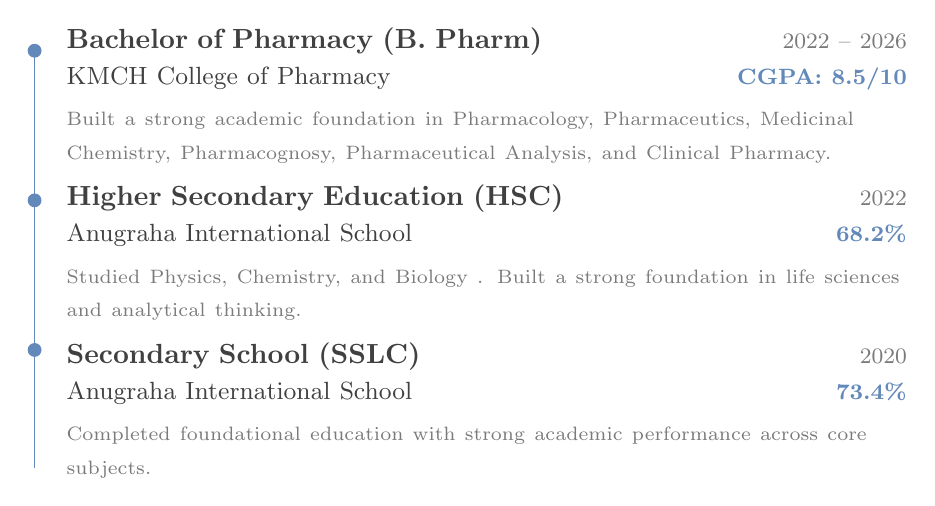
\begin{tikzpicture}[remember picture]

% Vertical line
\draw[mainblue, line width=0.6pt] (0.2,-0.3) -- (0.2,-5.6);

% Dots
\fill[mainblue] (0.2,-0.3) circle (2.5pt);
\fill[mainblue] (0.2,-2.2) circle (2.5pt);
\fill[mainblue] (0.2,-4.1) circle (2.5pt);

% ---------- UG ----------
\node[anchor=north west, inner sep=0, text width=0.88\textwidth] at (0.6, 0) {
    \textbf{\textcolor{darkgray}{Bachelor of Pharmacy (B. Pharm)}} \hfill \textcolor{textgray}{\footnotesize 2022 -- 2026}\\[1pt]
    {\small \textcolor{darkgray}{KMCH College of Pharmacy}} \hfill \textcolor{mainblue}{\footnotesize \textbf{CGPA: 8.5/10}}\\[3pt]
    {\scriptsize \textcolor{textgray}{
    Built a strong academic foundation in Pharmacology, Pharmaceutics, Medicinal Chemistry, Pharmacognosy, Pharmaceutical Analysis, and Clinical Pharmacy.}}
};

% ---------- HSC ----------
\node[anchor=north west, inner sep=0, text width=0.88\textwidth] at (0.6, -2.0) {
    \textbf{\textcolor{darkgray}{Higher Secondary Education (HSC)}} \hfill \textcolor{textgray}{\footnotesize 2022}\\[1pt]
    {\small \textcolor{darkgray}{Anugraha International School }} \hfill \textcolor{mainblue}{\footnotesize \textbf{68.2\%}}\\[3pt]
    {\scriptsize \textcolor{textgray}{
    Studied Physics, Chemistry, and Biology . Built a strong foundation in life sciences and analytical thinking.}}
};

% ---------- SSLC ----------
\node[anchor=north west, inner sep=0, text width=0.88\textwidth] at (0.6, -4.0) {
    \textbf{\textcolor{darkgray}{Secondary School (SSLC)}} \hfill \textcolor{textgray}{\footnotesize 2020}\\[1pt]
    {\small \textcolor{darkgray}{Anugraha International School }} \hfill \textcolor{mainblue}{\footnotesize \textbf{73.4\%}}\\[3pt]
    {\scriptsize \textcolor{textgray}{
    Completed foundational education with strong academic performance across core subjects.}}
};


\end{tikzpicture}

    \vspace{0.6cm}

    % ================= PROJECTS SECTION =================
    \renewcommand{\secicon}{\faFlask}
    \section*{Projects}

    
\begin{tikzpicture}[remember picture]
    \fill[mainblue] (0.2,-0.3) circle (2.5pt);
    
    \node[anchor=north west, inner sep=0, text width=0.88\textwidth] at (0.6, 0) {
        \textbf{\textcolor{darkgray}{Formulation and Evaluation of Herbal Ointment}} \hfill \textcolor{textgray}{\footnotesize Final Year Project}\\[1pt]
        {\small \textcolor{darkgray}{Academic Project}}\\[3pt]
        {\scriptsize \textcolor{textgray}{Developed a novel herbal formulation possessing antimicrobial properties. Conducted extraction, formulation, and in vitro evaluation using agar well diffusion method. Documented stability studies under various temperature conditions.}}
    };
    \end{tikzpicture}

    \vspace{0.6cm}

    % ================= INTERNSHIPS SECTION =================
    \renewcommand{\secicon}{\faBriefcase}
    \section*{Internships}

    
\begin{tikzpicture}[remember picture]
    \fill[mainblue] (0.2,-0.3) circle (2.5pt);

    \node[anchor=north west, inner sep=0, text width=0.88\textwidth] at (0.6, 0) {
        \textbf{\textcolor{darkgray}{Industrial Training }} \hfill \textcolor{textgray}{\footnotesize Dec 2025 -- Jan 2026}\\[1pt]
        {\small \textcolor{darkgray}{MEDOPHARM PRIVATE LIMITED, CHENNAI}}\\[3pt]
        {\scriptsize \textcolor{textgray}{Observed manufacturing and packaging of solid dosage forms. Gained knowledge in material flow and production instruments. Developed skills in QA, QC, R\&D, and documentation.}}
    };
    \end{tikzpicture}

    \vspace{0.6cm}

    % ================= CERTIFICATIONS SECTION =================
    \renewcommand{\secicon}{\faAward}
    \section*{Certifications}

    
\begin{tikzpicture}[remember picture]
    \draw[mainblue, line width=0.6pt] (0.2,-0.3) -- (0.2,-3.6);
    \fill[mainblue] (0.2,-0.3) circle (2.5pt);
    \fill[mainblue] (0.2,-1.4) circle (2.5pt);
    \fill[mainblue] (0.2,-2.5) circle (2.5pt);
    \fill[mainblue] (0.2,-3.6) circle (2.5pt);

    \node[anchor=north west, inner sep=0, text width=0.88\textwidth] at (0.6, 0) {
        \textbf{\textcolor{darkgray}{Certificate in Pharmacovigilance}} \hfill \textcolor{mainblue}{\footnotesize \textbf{2025}}\\[2pt]
        {\scriptsize \textcolor{textgray}{Coursera / Verified Certificate}}
    };

    \node[anchor=north west, inner sep=0, text width=0.88\textwidth] at (0.6, -1.1) {
        \textbf{\textcolor{darkgray}{Good Clinical Practice (GCP)}} \hfill \textcolor{mainblue}{\footnotesize \textbf{2024}}\\[2pt]
        {\scriptsize \textcolor{textgray}{NIDA Clinical Trials Network}}
    };

    \node[anchor=north west, inner sep=0, text width=0.88\textwidth] at (0.6, -2.2) {
        \textbf{\textcolor{darkgray}{Advanced First Aid \& CPR}} \hfill \textcolor{mainblue}{\footnotesize \textbf{2023}}\\[2pt]
        {\scriptsize \textcolor{textgray}{Indian Red Cross Society}}
    };
    
    \node[anchor=north west, inner sep=0, text width=0.88\textwidth] at (0.6, -3.3) {
        \textbf{\textcolor{darkgray}{Drug Regulatory Affairs \& QA}} \hfill \textcolor{mainblue}{\footnotesize \textbf{2023}}\\[2pt]
        {\scriptsize \textcolor{textgray}{Online Workshop / PharmaHub}}
    };
    \end{tikzpicture}

    \vspace{0.6cm}

    % ================= REFERENCES SECTION =================
    \renewcommand{\secicon}{\faBook}
    \section*{References}

    \begin{minipage}[t]{0.45\textwidth}
        \textbf{\textcolor{darkgray}{Dr. A. Rajasekaran}}\\[0.05cm]
        \textcolor{textgray}{Principal / KMCH Pharmacy}\\[0.15cm]
        {\scriptsize \textcolor{textgray}{\textbf{Phone:} +91 XXXXX XXXXX}}\\[0.05cm]
        {\scriptsize \textcolor{textgray}{\textbf{Email:} pharmacy@kmch.ac.in}}
    \end{minipage}
    \hfill
    \begin{minipage}[t]{0.45\textwidth}
        \textbf{\textcolor{darkgray}{Dr. R. Gayathri}}\\[0.05cm]
        \textcolor{textgray}{Professor / KMCH Pharmacy}\\[0.15cm]
        {\scriptsize \textcolor{textgray}{\textbf{Phone:} +91 9786110829}}\\[0.05cm]
        {\scriptsize \textcolor{textgray}{\textbf{Email:} r.kumar@kmch.ac.in}}
    \end{minipage}

\end{minipage}

\end{document}
